\documentclass{standalone}

\begin{document}


\subsubsection[Matrix Product]{Matrix Product}\label{NN:gemm}

Despite the mathematical formulation of the model we have to take into account also an efficient implementation.
From a numerical point-of-view we can notice that all the computation required by this kind of Networks (or layer if we consider it into an hybrid Neural Network architecture as we will see in the next sections) can be summarized into the matrix product evaluation.
The matrix product is a well-known numerical problem and its algorithmic complexity can be hardly reduced under $O(N^3)$\footnote{
  The complexity is often given in the assumption of only square matrices $(N\times N)$ involved in the computation.
  For no-square matrix the algorithm complexity is given by the product of the three possible different matrix dimensions involved ($(N\times K) = (N\times M)(M\times K)$ brings to $O(NMK)$ complexity).
  More sophisticated implementation of the algorithm are able to reduce the algorithm complexity (e.g Strassen algorithm) but neither implementation is able to overcome the $O(N^{2.7})$ complexity up-to-now.
}.
A crucial role on this kind of algorithms is played by the cache accesses.
The CPU cache is the hardware cache used by the CPU to store small portion of data in order to reduce the average cost (in time or energy consumption) to data access from the main memory.
Cache optimization is one of the most difficult parts to perform writing an algorithm, but it leads to highest performance gains.

In the matrix product we have to multiply each row of a matrix $A$ by each column of a second matrix $B$.
We work in the assumption that each matrix is stored into an array of 1D or 2D without nested structures.
In this case we can access to a contiguous memory portion of the first matrix since each row is given by a series of sequential index locations (the row elements are given by $x[0], x[1], \dots, x[N]$).
This configuration allows the cache optimization in the access to the first matrix, since we can store in a small portion of cache memory a series of row elements and use them in a vectorization environment.

From the second matrix we have to extract the elements from each column.
This means that the elements are given by a discontinuous portion of memories (the column elements are given by $x[0], x[M], x[2M], \dots, x[N(M-1)]$).
In this case we can not insert a full column into the cache memory and in consequence we have a \emph{cache-miss} at each iteration\footnote{
  The \emph{cache-miss} happens when a required data can not be found into the cache and so its search has to be done in the main memory (RAM).
}.

The simple matrix product as given by row-column multiplication is already affected by an intrinsic numerical problem which can drastically affect its performances.
The simplest workaround of this issue is to perform a transposition of the second matrix to obtain a row-row matrix product\footnote{
  In the discussion we have silently ignored the problems of matrix storage and the cache optimization for the resulting matrix accesses but in the above discussion we want to focus only on the main problems raising from the matrix product.
}.
In this way both matrices can be accessed in a sequential order.
The total complexity of the computation increase to $O(N^2)$ (for the matrix transposition, in the better case) $+ O(N^3)$ (for matrix product) but the numerical performances increase due to the cache-miss minimization\footnote{
  The cache memory is a very tight portion of memory and it is impossible to completely remove cache-misses.
}.

Following back to our Neural Network implementation we can obtain the output values using the above technique.
Moreover, we can assume from the beginning that the transposition of weight matrix and so remove the $O(N^2)$ calculus from the matrix product.
This simple (but carefully studied) optimization allows to obtain better results in the feed-forward evaluation, but it paybacks a revision of the standard mathematical formulation and a carefully implementation of the code.

\begin{figure}[htbp]
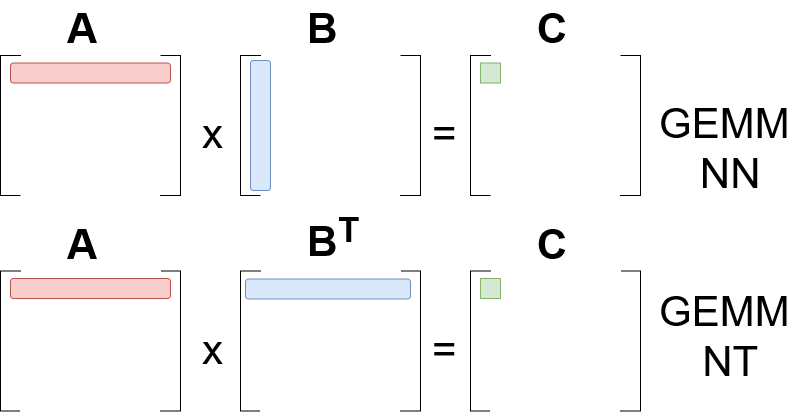
\includegraphics[width=0.45\textwidth]{GEMM_schema.png}
\quad
\centering
\def\svgwidth{0.45\textwidth}
\documentclass{standalone}

\begin{document}


\subsubsection[Matrix Product]{Matrix Product}\label{NN:gemm}

Despite the mathematical formulation of the model we have to take in count also an efficient implementation.
From a numerical point-of-view we can notice that all the computation required by this kind of Networks (or layer if we consider it into an hybrid Neural Network architecture as we will see in the next sections) can be summarized into the matrix product evaluation.
The matrix product is a well-known numerical problems and the complexity of the algorithm can be hardly reduced under $O(N^3)$\footnote{
  The complexity is often given in the assumption of only square matrices $(N\times N)$ involved in the computation.
  For no-square matrix the algorithm complexity is given by the product of the three possible different matrix dimensions involved ($(N\times K) = (N\times M)(M\times K)$ brings to $O(NMK)$ complexity).
  More sophisticated implementation of the algorithm are able to reduce the algorithm complexity (e.g Strassen algorithm) but neither implementation is able to overcome the $O(N^{2.7})$ complexity up-to-now.
}.
A crucial role on this kind of algorithms is played by the cache accesses.
The CPU cache is the hardware cache used by the CPU to store small portion of data in order to reduce the average cost (in time or energy consumption) to data access from the main memory.
Cache optimization is one of the most difficult parts to perform writing an algorithm, but can lead to highest performance gains.

In the matrix product we have to multiply each row of a matrix $A$ by each column of a second matrix $B$.
We work in the assumption that each matrix is stored into an array of 1D or 2D without nested structures.
In this case we can access to a contiguous memory portion of the first matrix since each row will be given by a series of sequential index locations (the row elements will be given by $x[0], x[1], \dots, x[N]$).
This configuration allows the cache optimization in the access to the first matrix since we can store in the small portion of cache memory a series of row elements and use them in a vectorization environment.

From the second matrix we have to extract the elements from each column.
This means that the elements will be given by a discontinuous portion of memories (the column elements will be given by $x[0], x[M], x[2M], \dots, x[N(M-1)]$).
In this case we can not insert a full column into the cache memory and in consequence we will have a \emph{cache-miss} at each iteration\footnote{
  The \emph{cache-miss} happens when a required data can not be found into the cache and so its search has to be done in the main memory (RAM).
}.

The simple matrix product as given by row-column multiplication is already affected by an intrinsic numerical problem which can drastically affect its performances.
The simplest workaround of this problem is to perform a transposition of the second matrix to obtain a row-row matrix product\footnote{
  In the discussion we have silently ignored the problems of matrix storage and the cache optimization for the resulting matrix accesses but in the above discussion we want to focus only on the main problems raising from the matrix product.
}.
In this way both matrices can be accessed in a sequential order.
The total complexity of the computation increase to $O(N^2)$ (for the matrix transposition, in the better case) $+ O(N^3)$ (for matrix product) but the numerical performances increase due to the cache-miss minimization\footnote{
  The cache memory is a very tight portion of memory and it is impossible to completely remove cache-misses.
}.

Following back to our Neural Network implementation we can obtain the output values using the above technique.
Moreover we can assumes from the beginning that the weight matrix is transposed and so remove the transposition step from the matrix product.
This simple (but carefully studied) optimization allows us to obtain better results in the feed-forward evaluation but it paybacks a revision of the standard mathematical formulation and a carefully implementation of the code.

\begin{figure}[htbp]
\includegraphics[width=0.45\textwidth]{gemm_schema.png}
\quad
\centering
\def\svgwidth{0.45\textwidth}
\documentclass{standalone}

\begin{document}


\subsubsection[Matrix Product]{Matrix Product}\label{NN:gemm}

Despite the mathematical formulation of the model we have to take in count also an efficient implementation.
From a numerical point-of-view we can notice that all the computation required by this kind of Networks (or layer if we consider it into an hybrid Neural Network architecture as we will see in the next sections) can be summarized into the matrix product evaluation.
The matrix product is a well-known numerical problems and the complexity of the algorithm can be hardly reduced under $O(N^3)$\footnote{
  The complexity is often given in the assumption of only square matrices $(N\times N)$ involved in the computation.
  For no-square matrix the algorithm complexity is given by the product of the three possible different matrix dimensions involved ($(N\times K) = (N\times M)(M\times K)$ brings to $O(NMK)$ complexity).
  More sophisticated implementation of the algorithm are able to reduce the algorithm complexity (e.g Strassen algorithm) but neither implementation is able to overcome the $O(N^{2.7})$ complexity up-to-now.
}.
A crucial role on this kind of algorithms is played by the cache accesses.
The CPU cache is the hardware cache used by the CPU to store small portion of data in order to reduce the average cost (in time or energy consumption) to data access from the main memory.
Cache optimization is one of the most difficult parts to perform writing an algorithm, but can lead to highest performance gains.

In the matrix product we have to multiply each row of a matrix $A$ by each column of a second matrix $B$.
We work in the assumption that each matrix is stored into an array of 1D or 2D without nested structures.
In this case we can access to a contiguous memory portion of the first matrix since each row will be given by a series of sequential index locations (the row elements will be given by $x[0], x[1], \dots, x[N]$).
This configuration allows the cache optimization in the access to the first matrix since we can store in the small portion of cache memory a series of row elements and use them in a vectorization environment.

From the second matrix we have to extract the elements from each column.
This means that the elements will be given by a discontinuous portion of memories (the column elements will be given by $x[0], x[M], x[2M], \dots, x[N(M-1)]$).
In this case we can not insert a full column into the cache memory and in consequence we will have a \emph{cache-miss} at each iteration\footnote{
  The \emph{cache-miss} happens when a required data can not be found into the cache and so its search has to be done in the main memory (RAM).
}.

The simple matrix product as given by row-column multiplication is already affected by an intrinsic numerical problem which can drastically affect its performances.
The simplest workaround of this problem is to perform a transposition of the second matrix to obtain a row-row matrix product\footnote{
  In the discussion we have silently ignored the problems of matrix storage and the cache optimization for the resulting matrix accesses but in the above discussion we want to focus only on the main problems raising from the matrix product.
}.
In this way both matrices can be accessed in a sequential order.
The total complexity of the computation increase to $O(N^2)$ (for the matrix transposition, in the better case) $+ O(N^3)$ (for matrix product) but the numerical performances increase due to the cache-miss minimization\footnote{
  The cache memory is a very tight portion of memory and it is impossible to completely remove cache-misses.
}.

Following back to our Neural Network implementation we can obtain the output values using the above technique.
Moreover we can assumes from the beginning that the weight matrix is transposed and so remove the transposition step from the matrix product.
This simple (but carefully studied) optimization allows us to obtain better results in the feed-forward evaluation but it paybacks a revision of the standard mathematical formulation and a carefully implementation of the code.

\begin{figure}[htbp]
\includegraphics[width=0.45\textwidth]{gemm_schema.png}
\quad
\centering
\def\svgwidth{0.45\textwidth}
\documentclass{standalone}

\begin{document}


\subsubsection[Matrix Product]{Matrix Product}\label{NN:gemm}

Despite the mathematical formulation of the model we have to take in count also an efficient implementation.
From a numerical point-of-view we can notice that all the computation required by this kind of Networks (or layer if we consider it into an hybrid Neural Network architecture as we will see in the next sections) can be summarized into the matrix product evaluation.
The matrix product is a well-known numerical problems and the complexity of the algorithm can be hardly reduced under $O(N^3)$\footnote{
  The complexity is often given in the assumption of only square matrices $(N\times N)$ involved in the computation.
  For no-square matrix the algorithm complexity is given by the product of the three possible different matrix dimensions involved ($(N\times K) = (N\times M)(M\times K)$ brings to $O(NMK)$ complexity).
  More sophisticated implementation of the algorithm are able to reduce the algorithm complexity (e.g Strassen algorithm) but neither implementation is able to overcome the $O(N^{2.7})$ complexity up-to-now.
}.
A crucial role on this kind of algorithms is played by the cache accesses.
The CPU cache is the hardware cache used by the CPU to store small portion of data in order to reduce the average cost (in time or energy consumption) to data access from the main memory.
Cache optimization is one of the most difficult parts to perform writing an algorithm, but can lead to highest performance gains.

In the matrix product we have to multiply each row of a matrix $A$ by each column of a second matrix $B$.
We work in the assumption that each matrix is stored into an array of 1D or 2D without nested structures.
In this case we can access to a contiguous memory portion of the first matrix since each row will be given by a series of sequential index locations (the row elements will be given by $x[0], x[1], \dots, x[N]$).
This configuration allows the cache optimization in the access to the first matrix since we can store in the small portion of cache memory a series of row elements and use them in a vectorization environment.

From the second matrix we have to extract the elements from each column.
This means that the elements will be given by a discontinuous portion of memories (the column elements will be given by $x[0], x[M], x[2M], \dots, x[N(M-1)]$).
In this case we can not insert a full column into the cache memory and in consequence we will have a \emph{cache-miss} at each iteration\footnote{
  The \emph{cache-miss} happens when a required data can not be found into the cache and so its search has to be done in the main memory (RAM).
}.

The simple matrix product as given by row-column multiplication is already affected by an intrinsic numerical problem which can drastically affect its performances.
The simplest workaround of this problem is to perform a transposition of the second matrix to obtain a row-row matrix product\footnote{
  In the discussion we have silently ignored the problems of matrix storage and the cache optimization for the resulting matrix accesses but in the above discussion we want to focus only on the main problems raising from the matrix product.
}.
In this way both matrices can be accessed in a sequential order.
The total complexity of the computation increase to $O(N^2)$ (for the matrix transposition, in the better case) $+ O(N^3)$ (for matrix product) but the numerical performances increase due to the cache-miss minimization\footnote{
  The cache memory is a very tight portion of memory and it is impossible to completely remove cache-misses.
}.

Following back to our Neural Network implementation we can obtain the output values using the above technique.
Moreover we can assumes from the beginning that the weight matrix is transposed and so remove the transposition step from the matrix product.
This simple (but carefully studied) optimization allows us to obtain better results in the feed-forward evaluation but it paybacks a revision of the standard mathematical formulation and a carefully implementation of the code.

\begin{figure}[htbp]
\includegraphics[width=0.45\textwidth]{gemm_schema.png}
\quad
\centering
\def\svgwidth{0.45\textwidth}
\input{./img/gemm.pdf_tex}
\caption{GEMM algorithms time performances.
GEMM NN: matrix multiplication considering both the matrices in \quotes{normal} format, i.e $A\cdot B$.
GEMM NT: matrix multiplication considering the first matrix in \quotes{normal} format and the second one transposed, i.e $A\cdot B^T$.
We perform 100 tests of 1K runs each of both the gemm algorithms using the \textsf{einsum} function of Numpy library.
The values are rescaled according to the mean time of the GEMM NN algorithm.
}
\label{fig:gemm}
\end{figure}

In the proposed numerical implementations of this model we implement both the matrix product cases to compare the performance results.
We tested the two implementation inside Python using the \textsf{einsum} function provided by the Numpy package.
In particular we evaluate the timing performances over 1000 applications of two the gemm functions (GEMM NN, i.e considering both matrices in \quotes{normal} shapes; GEMM NT, i.e considering the first matrix as \quotes{normal} and the second transpose) considering matrices of shapes ($100\times100$).
We performed 500 run and we save the minimum time obtained over the 10 realizations.
In Fig.~\ref{fig:gemm} we show the results rescaled by the mean time of the GEMM NN algorithm (reference).
As can be seen in Fig.~\ref{fig:gemm} the speedup of the GEMM NT matrix is evident and it is always faster than GEMM NN algorithm with a maximum of 3.2x in the speedup.

In the Byron library implementation we provide a parallelized version of this algorithm with also an \textsf{avx} support.
In this way we could manually manage the register memory of the two matrices and obtain faster version of the GEMM algorithm (especially for dimensions proportional to powers of 2 which are very common in neural network models).

\end{document}

\caption{GEMM algorithms time performances.
GEMM NN: matrix multiplication considering both the matrices in \quotes{normal} format, i.e $A\cdot B$.
GEMM NT: matrix multiplication considering the first matrix in \quotes{normal} format and the second one transposed, i.e $A\cdot B^T$.
We perform 100 tests of 1K runs each of both the gemm algorithms using the \textsf{einsum} function of Numpy library.
The values are rescaled according to the mean time of the GEMM NN algorithm.
}
\label{fig:gemm}
\end{figure}

In the proposed numerical implementations of this model we implement both the matrix product cases to compare the performance results.
We tested the two implementation inside Python using the \textsf{einsum} function provided by the Numpy package.
In particular we evaluate the timing performances over 1000 applications of two the gemm functions (GEMM NN, i.e considering both matrices in \quotes{normal} shapes; GEMM NT, i.e considering the first matrix as \quotes{normal} and the second transpose) considering matrices of shapes ($100\times100$).
We performed 500 run and we save the minimum time obtained over the 10 realizations.
In Fig.~\ref{fig:gemm} we show the results rescaled by the mean time of the GEMM NN algorithm (reference).
As can be seen in Fig.~\ref{fig:gemm} the speedup of the GEMM NT matrix is evident and it is always faster than GEMM NN algorithm with a maximum of 3.2x in the speedup.

In the Byron library implementation we provide a parallelized version of this algorithm with also an \textsf{avx} support.
In this way we could manually manage the register memory of the two matrices and obtain faster version of the GEMM algorithm (especially for dimensions proportional to powers of 2 which are very common in neural network models).

\end{document}

\caption{GEMM algorithms time performances.
GEMM NN: matrix multiplication considering both the matrices in \quotes{normal} format, i.e $A\cdot B$.
GEMM NT: matrix multiplication considering the first matrix in \quotes{normal} format and the second one transposed, i.e $A\cdot B^T$.
We perform 100 tests of 1K runs each of both the gemm algorithms using the \textsf{einsum} function of Numpy library.
The values are rescaled according to the mean time of the GEMM NN algorithm.
}
\label{fig:gemm}
\end{figure}

In the proposed numerical implementations of this model we implement both the matrix product cases to compare the performance results.
We tested the two implementation inside Python using the \textsf{einsum} function provided by the Numpy package.
In particular we evaluate the timing performances over 1000 applications of two the gemm functions (GEMM NN, i.e considering both matrices in \quotes{normal} shapes; GEMM NT, i.e considering the first matrix as \quotes{normal} and the second transpose) considering matrices of shapes ($100\times100$).
We performed 500 run and we save the minimum time obtained over the 10 realizations.
In Fig.~\ref{fig:gemm} we show the results rescaled by the mean time of the GEMM NN algorithm (reference).
As can be seen in Fig.~\ref{fig:gemm} the speedup of the GEMM NT matrix is evident and it is always faster than GEMM NN algorithm with a maximum of 3.2x in the speedup.

In the Byron library implementation we provide a parallelized version of this algorithm with also an \textsf{avx} support.
In this way we could manually manage the register memory of the two matrices and obtain faster version of the GEMM algorithm (especially for dimensions proportional to powers of 2 which are very common in neural network models).

\end{document}

\caption{GEMM algorithms time performances.
\textsf{GEMM NN}: matrix multiplication considering both the matrices in \quotes{normal} format, i.e $A\cdot B$.
\textsf{GEMM NT}: matrix multiplication considering the first matrix in \quotes{normal} format and the second one transposed, i.e $A\cdot B^T$.
We perform 100 tests of 1K runs each of both the \textsf{GEMM} algorithms using the \textsf{einsum} function of \textsf{Numpy} library.
The values are rescaled according to the mean time of the \textsf{GEMM NN} algorithm.
}
\label{fig:gemm}
\end{figure}

In the proposed numerical implementations of this model we implement both the matrix product cases to compare the performance results.
We tested the two implementations inside \textsf{Python} using the \textsf{einsum} function provided by the \textsf{Numpy} package.
In particular, we evaluated the time-performances over 1000 applications of the two \textsf{GEMM} functions (\textsf{GEMM NN}, i.e considering both matrices with \quotes{normal} shapes; \textsf{GEMM NT}, i.e considering the first matrix as \quotes{normal} and the second transposed) considering matrices of shapes ($100\times100$).
We performed $500$ run and we saved the minimum time obtained over $10$ realizations.
In Fig.~\ref{fig:gemm} we show the results rescaled by the mean time (over the 500 realizations) of the \textsf{GEMM NN} algorithm (reference).
As can be seen in Fig.~\ref{fig:gemm} the speedup of the \textsf{GEMM NT} matrix is evident and it is always faster than \textsf{GEMM NN} algorithm with a maximum of $3.2$x in the speedup.

In the \textsf{Byron} library we provide a parallelized version of this algorithm with also an \textsf{avx} support.
In this way we could manually manage the register memory of the two matrices and obtain a faster \textsf{GEMM} algorithm (especially for dimensions proportional to powers of 2 which are very common in neural network models).

\end{document}
